Our project includes four view, paper view, paper details view, author view, and keyword view.
\subsection{Paper view}
In paper view, we have we show all the papers, grouped by year. Each year occupies one column. This view is scroll-able horizontally to zoom in/out the view. Zoom in/out button is provided on the left top as well.

Papers' title appears on one row and be click-able. When a paper is clicked on, the papers that this paper cites and the ones that cite it will be highlighted with different color. Curved links are display to show the relationship between papers. Moreover, when a paper is mouse over, a pop-up will show the paper's full title, author lists. 

This whole paper view can be sorted either alphabetically or by citation count. We provide a checkbox to display/hide citation count bar. The citation bar appears right under each paper's title, the length of which is proportional to the paper's number of citations and scaled within the year, because it is unfair to compare two papers published in different years. This help the user identify influential papers at a glance.

There are also two search buttons, which allows user to search author name or paper title. If more than papers are returned, all of them will be highlighted as black. If only return one result, the result will set as selected paper and showing its reference.

Once paper is selected, paper details and author view will be updated correspondingly based on the selection.

\subsection{Paper details view}
Paper view shows all details about the selected paper, including title, authors, abstract, keywords, cited count, year, and its external link, which points to ACM web-site.

Keywords are click-able. Once keywords is clicked, it will be set as "selected" and update keyword view.

Also, in order to give users a brief idea about reference information, a subset paper view is added here, which only displays the highlighted papers in the paper view. Titles here also can be enlarged when mouse over it.

\subsection{Author view}

Author view only displays the selected paper, its authors, and its authors' publications. Each green circle represents one paper and is scaled by its cited count.  Even though it is a much smaller set compared with original one, the view allows user to click and change the selected papers with transition. 

When users mouse-over it, a tool-tip will show on the right bottom to show published year and cited count. In the mean time, other unconnected nodes will be transparent so to highlight mouse-over-ed paper and its author or  mouse-over-ed author and all his/her publications.

\subsection{Keyword view}
In this view we display all the keywords extracted from our paper database. Since the number of keywords are large (we have nearly a thousand keywords), we opted for a simple view where the keywords are sorted in alphabetical order and shown in a grid. Some keywords are long and will thus be truncated in the view, but will be shown in full when the user moves the mouse over. We achieved this by fading out the two adjacent keywords. The list of keywords can be filtered using a search box (irrelevant keywords will be grayed out). Keywords are clickable. When a keyword is clicked on, it will be highlighted, together with all its related keywords. Two keywords are related if they appear together in more than one papers (Figure \ref{fig:kw_selected}).

\begin{figure}[ht]			
    \centering
    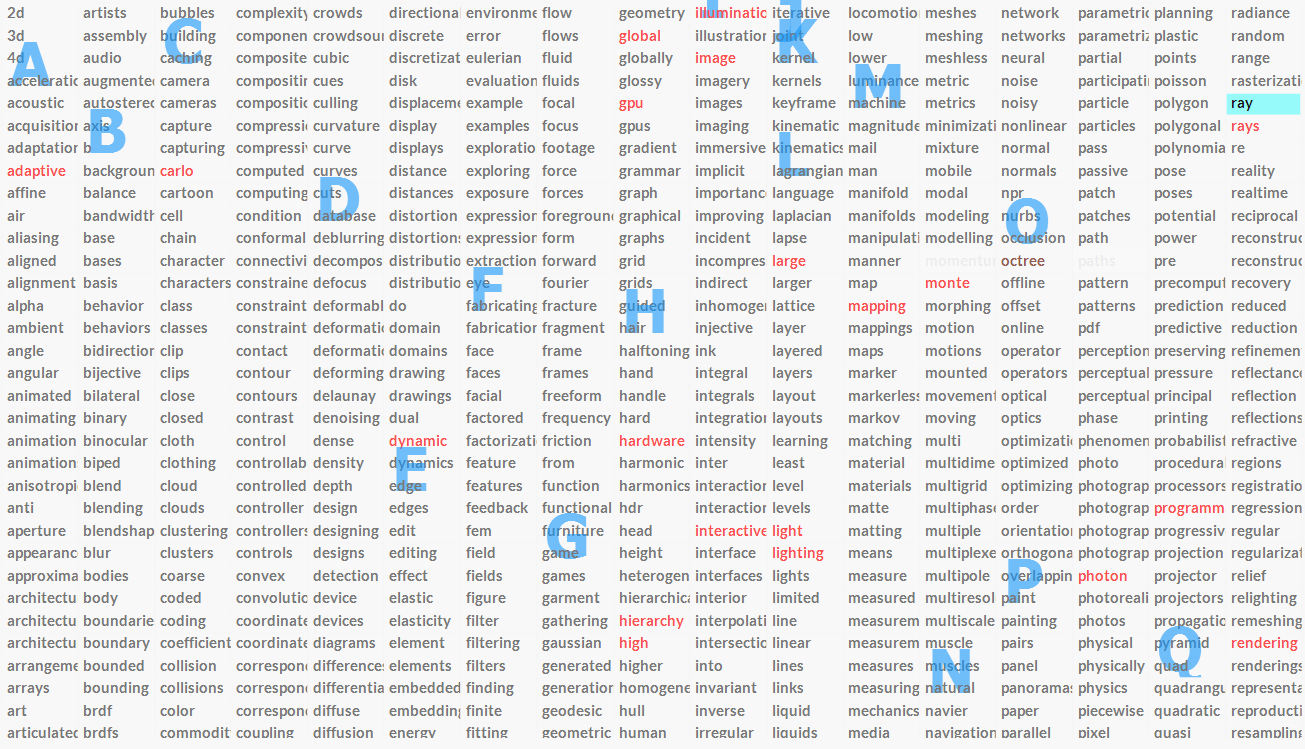
\includegraphics[width=0.7\textwidth]{keyword_view_selected.png}
    \caption{Keyword view with a keyword selected}
    \label{fig:kw_selected}
\end{figure}

Selecting a set of keywords will have an effect on the paper view. Papers having all the selected keywords will be highlighted. This is very useful for exploration of the paper database based on keywords.
